\documentclass[a4paper,12pt]{article}
	
\usepackage[T2A]{fontenc}			
\usepackage[utf8]{inputenc}			
\usepackage[english,russian]{babel}	

\usepackage[
bookmarks=true, colorlinks=true, unicode=true,
urlcolor=black,linkcolor=black, anchorcolor=black,
citecolor=black, menucolor=black, filecolor=black,
]{hyperref}

\usepackage{color}
\usepackage{caption}


\usepackage{amsmath,amsfonts,amssymb,amsthm,mathtools} 
\usepackage{wasysym}

\usepackage{graphicx}
%\usepackage[cache=false]{minted}
\usepackage{cmap}
\usepackage{indentfirst}

\usepackage{listings} 
\usepackage{fancyvrb}
\usepackage{slashbox}

\usepackage{geometry}
\geometry{left=2cm}
\geometry{right=1.5cm}
\geometry{top=1cm}
\geometry{bottom=2cm}

\setlength{\parindent}{5ex}
\setlength{\parskip}{0.5em}

\usepackage{titlesec}
\usepackage{pgfplots}
\usepackage{filecontents}
\usetikzlibrary{datavisualization}
\usetikzlibrary{datavisualization.formats.functions}

\DeclareCaptionFont{white}{\color{white}}
\DeclareCaptionFormat{listing}{\colorbox{gray}{\parbox{\textwidth}{#1#2#3}}}
\captionsetup[lstlisting]{format=listing,labelfont=white,textfont=white}
\lstloadlanguages{% Check Dokumentation for further languages ...
C,
C++,
csh,
Java
}

\definecolor{red}{rgb}{0.6,0,0} % for strings
\definecolor{blue}{rgb}{0,0,0.6}
\definecolor{green}{rgb}{0,0.8,0}
\definecolor{cyan}{rgb}{0.0,0.6,0.6}

\lstset{ %
language=Lisp,                 % выбор языка для подсветки
basicstyle=\small\sffamily, % размер и начертание шрифта для подсветки кода
numbers=left,               % где поставить нумерацию строк (слева\справа)
numberstyle=\tiny,           % размер шрифта для номеров строк
stepnumber=1,                   % размер шага между двумя номерами строк
numbersep=5pt,                % как далеко отстоят номера строк от подсвечиваемого кода
showspaces=false,
backgroundcolor=\color{white},         
showstringspaces=false,      % показывать или нет пробелы в строках
showtabs=false,             % показывать или нет табуляцию в строках
frame=single,              % рисовать рамку вокруг кода
tabsize=2,                 % размер табуляции по умолчанию равен 2 пробелам
captionpos=t,              % позиция заголовка вверху [t] или внизу [b] 
breaklines=true,           % автоматически переносить строки (да\нет)
breakatwhitespace=false, % переносить строки только если есть пробел
escapeinside={\%*}{*)}
}

% Для измененных титулов глав:
\definecolor{gray75}{gray}{0.75} % определяем цвет
\newcommand{\hsp}{\hspace{20pt}} % длина линии в 20pt
% titleformat определяет стиль
\titleformat{\chapter}[hang]{\Huge\bfseries}{\thechapter\hsp\textcolor{gray75}{|}\hsp}{0pt}{\Huge\bfseries}

\begin{document}
	
\begin{figure}[h!]
	\begin{center}
		{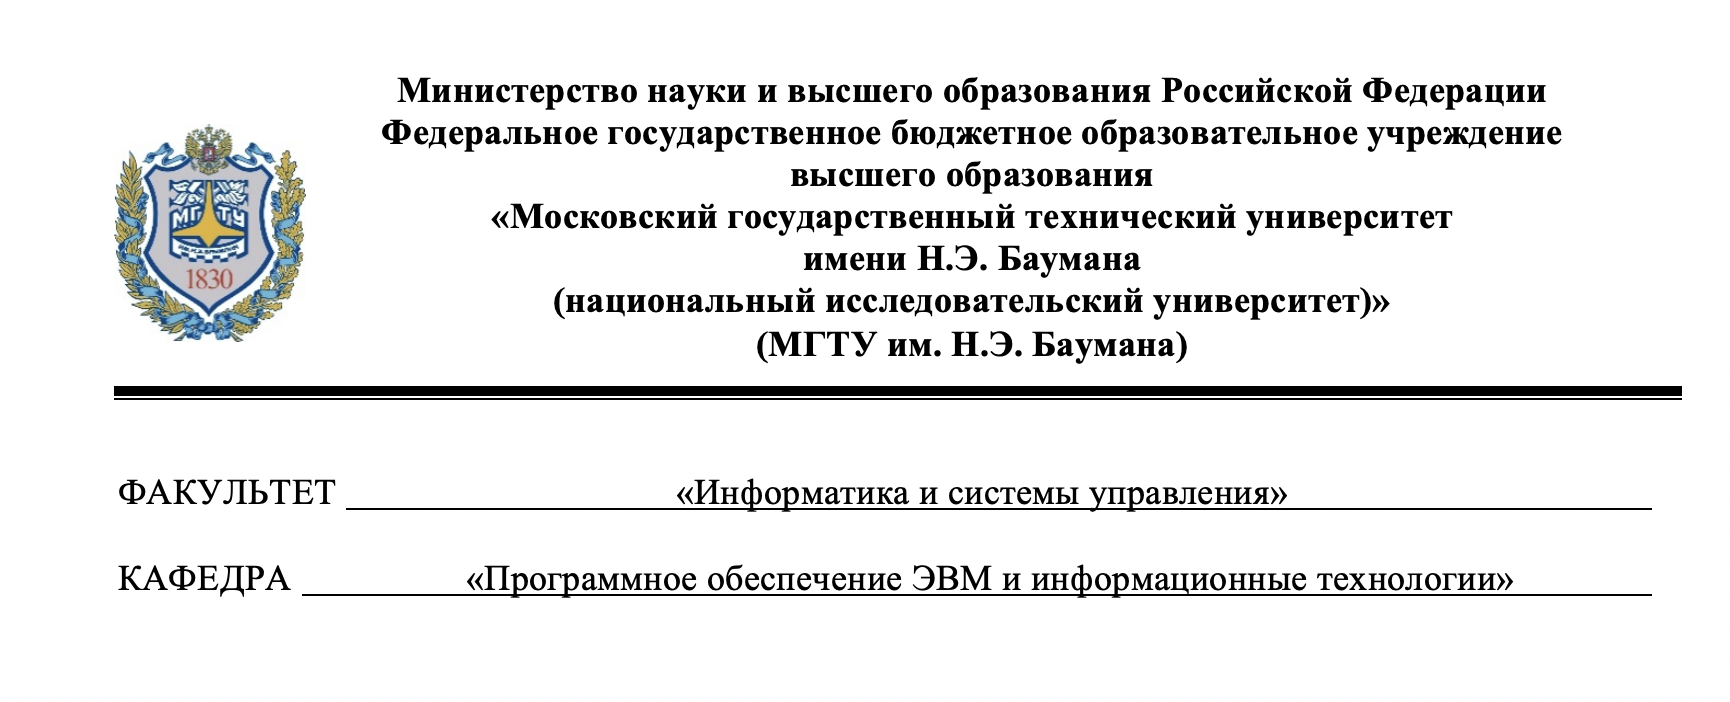
\includegraphics[width = \textwidth]{titul.png}}
	\end{center}
\end{figure}

\vspace*{20mm}

\huge
\begin{center}
	Лабораторная работа №3
\end{center}


\vspace*{50mm}

\large
\begin{flushleft}
	Студент: Луговой Д.М. \\
	Группа: ИУ7-61Б \\
	Преподаватель: Толпинская Н.Б.
\end{flushleft}

\vspace*{60mm}

\large
\begin{center}
	Москва, 2020 г.
\end{center}

\thispagestyle{empty}

\newpage
\vspace*{10mm}
\textbf{Цель работы}: приобрести навыки создания и использования функций пользователя в Lisp.\\

\textbf{Задачи работы}: изучить способы создания и использования именованных и неименованных функций пользователя для обработки списков.

\begin{enumerate}

\item \textbf{Базис LISP}

Базис языка – это необходимый минимальный набор конструкций, которые должные обязательно присутствовать, чтобы при их помощи составлять команды. Базис языка Lisp образуют атомы, структуры, базовые функции и функционалы. 

\item \textbf{Классификация функций}

Функция есть однозначное отображение множества исходных данных на множество её значений.
Функции классифицируются на:
\begin{itemize}
\item Чистые математические функции - принимают фиксированное количество аргументов
\item Формы – принимают не фиксированное количество аргументов или обрабатывают аргументы по разному
\item Функционалы (высших порядков) – используют другие функции в качестве аргументов или вырабатывают в качестве результатов.
\item Базисные функции
\begin{itemize}
\item Селекторы (функции доступа) - car, cdr
\item Конструкторы (функции создания структур) - cons, list
\item Предикаты - atom, null, listp, consp
\item Функции сравнения - eq, eql, equal, =, equalp
\end{itemize}
\end{itemize}

\item \textbf{Работа функций CAR и CDR}

CAR и CDR являются базовыми функциями доступа к данным. CAR принимает точечную пару или пустой список в качестве аргумента и возвращает первый элемент или nil, соответственно. CDR принимает точечную пару или пустой список и возвращает список состоящий из всех элементов, кроме первого. Если в списке меньше двух элементов, то возвращается Nil.

\item \textbf{Различия функций CONS и LIST}

LIST и CONS являются функциями создания списков.
Функция cons принимает 2 аргумента и создает списочную ячейку, указатель головы которой указывает на 1-ый аргумент, а указатель хвоста - на 2-ой элемент. Функция list принимает переменное число аргументов и возвращает список, элементы которого – переданные в функцию аргументы.\\

\end{enumerate}

{\LARGE Задание №1}\\

Составить диаграмму вычисления следующих выражений:
\begin{enumerate}
\item (equal 3 (abs - 3))
\begin{figure}[ht!]
\center{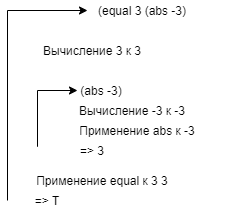
\includegraphics[scale=0.8]{FaLP1.png}}
\end{figure}
\item (equal (+ 1 2) 3)
\begin{figure}[ht!]
\center{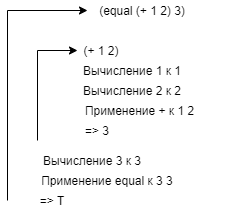
\includegraphics[scale=0.8]{FaLP2.png}}
\end{figure}
\newpage
\item (equal (* 4 7) 21)
\begin{figure}[ht!]
\center{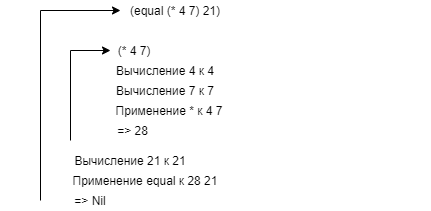
\includegraphics[scale=0.8]{FaLP3.png}}
\end{figure}
\item (equal (* 2 3) (+ 7 2))
\begin{figure}[ht!]
\center{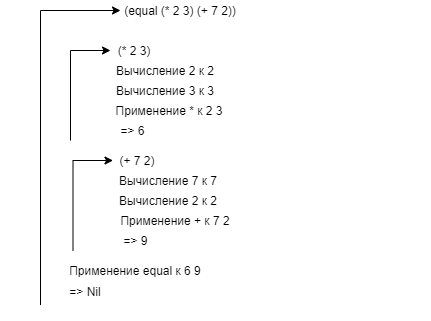
\includegraphics[scale=0.8]{FaLP4.png}}
\end{figure}
\newpage
\item (equal (- 7 3) (* 3 2))
\begin{figure}[ht!]
\center{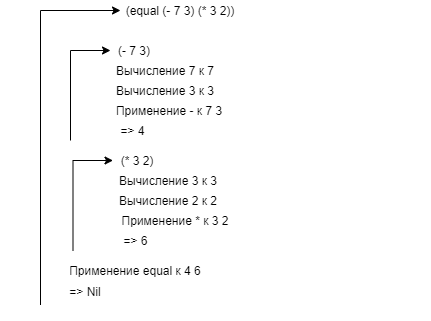
\includegraphics[scale=0.8]{FaLP5.png}}
\end{figure}
\item (equal (abs (- 2 4)) 3))\\
\begin{figure}[ht!]
\center{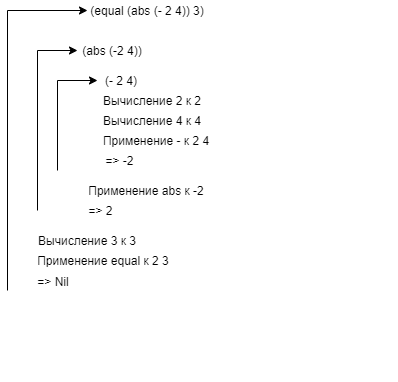
\includegraphics[scale=0.8]{FaLP6.png}}
\end{figure}
\end{enumerate}

\newpage
\vspace*{10mm}
{\LARGE Задание №2}\\

Написать функцию, вычисляющую гипотенузу прямоугольного треугольника по заданным катетам и составить диаграмму её вычисления.

(defun hyp (a b) (sqrt (+ (* a a) (* b b))))

Пример: (hyp 3 4) -> 5.0
\begin{figure}[ht!]
\center{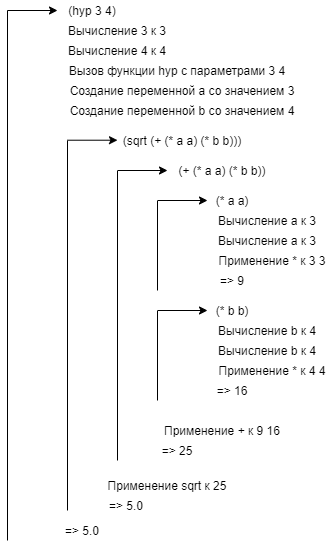
\includegraphics[scale=0.8]{FaLP7.png}}
\end{figure}

\newpage
\vspace*{10mm}
{\LARGE Задание №3}\\

Написать функцию, вычисляющую объем параллелепипеда по 3-м его сторонам, и составить диаграмму ее вычисления.

(defun vol (a b h) (* a b h))

Пример (vol 1 2 3) -> 6

\begin{figure}[ht!]
\center{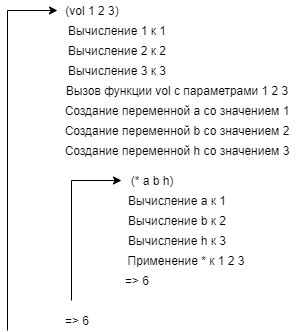
\includegraphics[scale=0.8]{FaLP8.png}}
\end{figure}

{\LARGE Задание №4}\\
Каковы результаты вычисления следующих выражений?

\begin{enumerate}
\item (list 'a 'b c)\\
Результат:The variable C is unbound, т.к. С нельзя вычислить.
\item (cons 'a (b c))\\
Результат:The variable C is unbound, т.к. С нельзя вычислить.
\item (cons 'a '(b c))\\
Результат:(A B C)
\item (caddr (1 2 3 4 5))\\
Результат:Illegal function call, т.к. 1 не является функцией.
\item (cons 'a 'b 'c)\\
Результат:Invalid number of arguments: 3, т.к. cons должен принимать 2 аргумента.
\item (list 'a (b c))\\
Результат:The variable C is unbound, т.к. С нельзя вычислить.
\item (list a '(b c))\\
Результат:The variable A is unbound, т.к. С нельзя вычислить.
\item (list (+ 1 '(length '(1 2 3))))\\
Результат:The value (LENGTH '(1 2 3)) is not of type NUMBER, т.к. '(LENGTH '(1 2 3)) не вычисляется из-за '.
\end{enumerate}

\vspace*{10mm}
{\LARGE Задание №5}\\

Написать функцию longer\_then от двух списков-аргументов, которая возвращает T, если первый аргумент имеет большую длину.

(defun longer\_then (a b) (> (length a) (length b)))

Пример: (longer\_then '(1 2) '(1 2 3 4)) -> NIL\\

{\LARGE Задание №6}\\

Каковы результаты вычисления следующих выражений?

\begin{enumerate}
\item (cons 3 (list 5 6))\\
Результат: (3 5 6)
\item (list 3 ‘from 9 ‘gives (- 9 3))\\
Результат: (3 FROM 9 GIVES 6)
\item (+ (length '(1 for 2 too)) (car ‘(21 22 23)))\\
Результат: 25
\item (cdr ‘(cons is short for ans))\\
Результат: (IS SHORT FOR ANS)
\item (car (list one two))\\
Результат: The variable ONE is unbound, т.к. ONE  нельзя вычислить.
\item (cons 3 ‘(list 5 6))\\
Результат: (3 LIST 5 6)
\item (car (list ‘one ‘two))\\
Результат: ONE\\
\end{enumerate}

\vspace*{10mm}
{\LARGE Задание №7}\\

Дана функция (defun mystery (x) (list (second x) (first x))). Какие результаты вычисления следующих выражений?

\begin{enumerate}
\item (mystery '(one two))\\
Результат: (TWO ONE)
\item (mystery 'free)\\
Результат: The value FREE is not of type LIST, т.е. free не список.
\item (mystery (last 'one 'two)\\
Результат: The value ONE is not of type LIST when binding LIST, т.е. one не список.
\item (mystery 'one 'two)\\
Результат: Invalid number of arguments: 2, т.к. функция принимает 1 аргумент.
\end{enumerate}

\end{document}

